\documentclass{article}
\usepackage{caption}
\usepackage{cancel}
\usepackage{tikz}
\usepackage{pifont}
\usepackage[fontsize=16pt]{fontsize}

\author{}
\date{}
\title{Simple\\Addition\\Course\\
\begin{center}
\includegraphics[width=4em]{ApS_logo.png}
\end{center}
\begin{normalsize}Tutoring Centre Ferndale\end{normalsize}}

\begin{document}
\maketitle

\section*{Addition}

\paragraph{Addition}
Addition means putting things together into a single amount.\\

\paragraph{Add}
Add just means to do addition.

\paragraph{Plus}
Plus means more, and in writing addition, the plus sign $+$ is used.

\paragraph{Sum}
The result of addition is called a sum.\\

2 + 3 = 5 means that 2 of something \ding{46}\ding{46} plus 3 of something \ding{46}\ding{46}\ding{46} 
makes a sum of 5 somethings \ding{46}\ding{46}\ding{46}\ding{46}\ding{46}

{\Large $$\underbrace{2}_{\textrm{\small{number}}} \overbrace{+}^{\textrm{\small{plus}}} \underbrace{3}_{\textrm{\small{number}}} = \overbrace{9}^{\textrm{\small{sum}}}$$}\\

\paragraph{Total}
When you add more than two numbers, the answer is called a total.

{\Large $$\underbrace{2}_{\textrm{\small{number}}} \overbrace{+}^{\textrm{\small{plus}}} \underbrace{3}_{\textrm{\small{number}}}  \overbrace{+}^{\textrm{\small{plus}}} \underbrace{4}_{\textrm{\small{number}}} = \overbrace{5}^{\textrm{\small{total}}}$$}

\newpage

\paragraph{Number Lines}
You can also use a number line to show what is happening. Moving to the right on the line represents adding:

\begin{center}
$$2+3=5$$
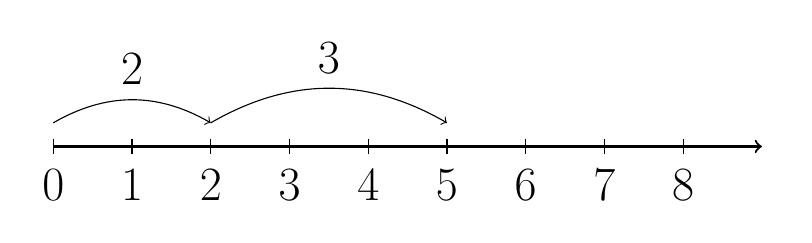
\begin{tikzpicture}
\draw[thick, ->] (0,0) -- (9,0) node[below] {$\ $};
\foreach \n in {0,1,2,3,4,5,6,7,8} {\draw (\n,0.1) -- (\n,-0.1) node[below] {$\n$};}
\draw[->, bend left=30] (0,0.3) to node[above] {$2$} (2,0.3);
\draw[->, bend left=30] (2,0.3) to node[above] {$3$} (5,0.3);
\end{tikzpicture}
\end{center}

\begin{enumerate}
\item What is addition?
\item What is adding?
\item What does plus mean?
\item What is a sum?
\item What is a total?
\item Put two things next to two more things and count them. What is the total?
\item Show $2+2=4$ on a number line.

\newpage

\section*{The Addition Table}
Learning addition starts with memorizing the sums of the single digit numbers. You need to learn all the sums from 1 + 1 to 9 + 9 and then you can easily add any list of numbers of any size.\\

\begin{table}[h]
\centering
\begin{tabular}{|l|l|l|l|l|l|l|l|l|l|}
\hline
+ & 1  & 2  & 3  & 4  & 5  & 6  & 7  & 8  & 9                       \\ \hline
1 & 2  & 3  & 4  & 5  & 6  & 7  & 8  & 9  & 10                      \\ \hline
2 & 3  & 4  & 5  & 6  & 7  & 8  & 9  & 10 & 11                      \\ \hline
3 & 4  & 5  & 6  & 7  & 8  & 9  & 10 & 11 & 12                      \\ \hline
4 & 5  & 6  & 7  & 8  & 9  & 10 & 11 & 12 & 13                      \\ \hline
5 & 6  & 7  & 8  & 9  & 10 & 11 & 12 & 13 & 14                      \\ \hline
6 & 7  & 8  & 9  & 10 & 11 & 12 & 13 & 14 & 15                      \\ \hline
7 & 8  & 9  & 10 & 11 & 12 & 13 & 14 & 15 & 16                      \\ \hline
8 & 9  & 10 & 11 & 12 & 13 & 14 & 15 & 16 & 17                      \\ \hline
9 & 10 & 11 & 12 & 13 & 14 & 15 & 16 & 17 & \multicolumn{1}{c|}{18} \\ \hline
\end{tabular}
\caption*{The Addition table}
\end{table}

\item Fill in the blank addition table.

\begin{table}[h]
\centering
\begin{tabular}{|l|l|l|l|l|l|l|l|l|l|}
\hline
+ & 1  & 2  & 3  & 4  & 5  & 6  & 7  & 8  & 9                       \\ \hline
1 &    &    &    &    &    &    &    &    &                         \\ \hline
2 &    &    &    &    &    &    &    &    &                         \\ \hline
3 &    &    &    &    &    &    &    &    &                         \\ \hline
4 &    &    &    &    &    &    &    &    &                         \\ \hline
5 &    &    &    &    &    &    &    &    &                         \\ \hline
6 &    &    &    &    &    &    &    &    &                         \\ \hline
7 &    &    &    &    &    &    &    &    &                         \\ \hline
8 &    &    &    &    &    &    &    &    &                         \\ \hline
9 &    &    &    &    &    &    &    &    & \multicolumn{1}{c|}{18} \\ \hline
\end{tabular}
\caption*{Fill in this blank Addition table}
\end{table}
\item Practice adding these single digits until you can do them all quickly and without having to think.

\newpage

\section*{Addition in columns}
Adding larger numbers is done by arranging the numbers into columns aligned at the right. Each column of digits, the ones, the tens, the hundreds and so on, is added separately to show a total.

\begin{center}
\begin{tabular}{c@{\,}c@{\,}c@{\,}}
 &7&2\\
+&2&4\\
\hline
=&9&6\\
\hline
\hline
\end{tabular}
\end{center}

The total is separated from the numbers being added by a single line, and is double underlined to indicate that this is a final answer.

Any number of numbers, of any length, can be added in this way.

Keeping the ones, tens, hundreds and so on all lined up under each other in neat columns is important and helps make sure that no mistakes are made.\\

\begin{center}
\begin{tabular}{c@{\,}c@{\,}c@{\,}c@{\,}c@{\,}c@{\,}c@{\,}c@{\,}}
 & &1&0&4,&2&1&3\\
 & & & &3,&1&1&2\\
 &1,&2&8&2,&2&3&1\\
+&1,&4&0&0,&3&1&1\\
\hline
=&2,&7&8&9,&8&6&7\\
\hline
\hline
\end{tabular}\\
\end{center}

\item Write 133, 21, and 44 under each other with their units and tens places lined up.
\item Write a plus sign to the left of the 44 to show that you are adding them.
\item Draw a line under these numbers.
\item Write the total of each column in the ones, tens and hundreds places.
\item Draw a double underline to show that this is the total.

\section*{Carrying}
Where the total of a column is greater than 9, because there is a tens digit to include now, totals must be made for each column that are then added to reach the final total.\\

\begin{center}
\begin{tabular}{c@{\,}c@{\,}c@{\,}c@{\,}c}
     &1,&2&3&4\\
     &3,&4&5&6\\
   + & &7&8&9\\
\hline
     & & &1&9\\
     & & 1&6&\\
     & 1& 3&&\\
     & 4& & &\\
\hline
     &5,&4&7&9\\
\hline
\hline
\end{tabular}\\
\end{center}

\vspace{28pt}
This is made shorter by "carrying" any tens digits over to the column to the left.\\

\begin{center}
\begin{tabular}{c@{\,}c@{\,}c@{\,}c@{\,}c}
	&1,&2&3&4\\
	&3,&4&5&6\\
  + & &7&8&9\\
	&\tiny{1}&\tiny{1}&\tiny{1}&\\
	\hline
	&5,&4&7&9\\
	\hline
	\hline
\end{tabular}
\end{center}

\item Write two numbers under each other with their digits lined up at the right, and draw a line under them.
\item Add up each column starting with the ones column on the right, and write any carries to be included in the next column.
\item Keep going until you have a total, and draw a double line under it.\\

Practice doing more addition with carrying:
\item What is 274 + 386 + 45?
\item What is 593 + 721 + 468?
\item What is 689 + 47 + 598?
\item What is 846 + 572 + 693?
\item What is 319 + 475 + 628?
    
\item Keep practicing adding numbers until you are getting right answers every time and you feel confident about it.\\

And that's how you do addition!\\

\end{enumerate}

\end{document}